% Options for packages loaded elsewhere
\PassOptionsToPackage{unicode}{hyperref}
\PassOptionsToPackage{hyphens}{url}
%
\documentclass[
  12pt,
]{article}
\usepackage{amsmath,amssymb}
\usepackage{lmodern}
\usepackage{ifxetex,ifluatex}
\ifnum 0\ifxetex 1\fi\ifluatex 1\fi=0 % if pdftex
  \usepackage[T1]{fontenc}
  \usepackage[utf8]{inputenc}
  \usepackage{textcomp} % provide euro and other symbols
\else % if luatex or xetex
  \usepackage{unicode-math}
  \defaultfontfeatures{Scale=MatchLowercase}
  \defaultfontfeatures[\rmfamily]{Ligatures=TeX,Scale=1}
\fi
% Use upquote if available, for straight quotes in verbatim environments
\IfFileExists{upquote.sty}{\usepackage{upquote}}{}
\IfFileExists{microtype.sty}{% use microtype if available
  \usepackage[]{microtype}
  \UseMicrotypeSet[protrusion]{basicmath} % disable protrusion for tt fonts
}{}
\makeatletter
\@ifundefined{KOMAClassName}{% if non-KOMA class
  \IfFileExists{parskip.sty}{%
    \usepackage{parskip}
  }{% else
    \setlength{\parindent}{0pt}
    \setlength{\parskip}{6pt plus 2pt minus 1pt}}
}{% if KOMA class
  \KOMAoptions{parskip=half}}
\makeatother
\usepackage{xcolor}
\IfFileExists{xurl.sty}{\usepackage{xurl}}{} % add URL line breaks if available
\IfFileExists{bookmark.sty}{\usepackage{bookmark}}{\usepackage{hyperref}}
\hypersetup{
  pdftitle={Lab 3 - Probability: Distributional Theory Continued},
  pdfauthor={Daniel Carpenter},
  hidelinks,
  pdfcreator={LaTeX via pandoc}}
\urlstyle{same} % disable monospaced font for URLs
\usepackage[margin=1in]{geometry}
\usepackage{color}
\usepackage{fancyvrb}
\newcommand{\VerbBar}{|}
\newcommand{\VERB}{\Verb[commandchars=\\\{\}]}
\DefineVerbatimEnvironment{Highlighting}{Verbatim}{commandchars=\\\{\}}
% Add ',fontsize=\small' for more characters per line
\usepackage{framed}
\definecolor{shadecolor}{RGB}{248,248,248}
\newenvironment{Shaded}{\begin{snugshade}}{\end{snugshade}}
\newcommand{\AlertTok}[1]{\textcolor[rgb]{0.94,0.16,0.16}{#1}}
\newcommand{\AnnotationTok}[1]{\textcolor[rgb]{0.56,0.35,0.01}{\textbf{\textit{#1}}}}
\newcommand{\AttributeTok}[1]{\textcolor[rgb]{0.77,0.63,0.00}{#1}}
\newcommand{\BaseNTok}[1]{\textcolor[rgb]{0.00,0.00,0.81}{#1}}
\newcommand{\BuiltInTok}[1]{#1}
\newcommand{\CharTok}[1]{\textcolor[rgb]{0.31,0.60,0.02}{#1}}
\newcommand{\CommentTok}[1]{\textcolor[rgb]{0.56,0.35,0.01}{\textit{#1}}}
\newcommand{\CommentVarTok}[1]{\textcolor[rgb]{0.56,0.35,0.01}{\textbf{\textit{#1}}}}
\newcommand{\ConstantTok}[1]{\textcolor[rgb]{0.00,0.00,0.00}{#1}}
\newcommand{\ControlFlowTok}[1]{\textcolor[rgb]{0.13,0.29,0.53}{\textbf{#1}}}
\newcommand{\DataTypeTok}[1]{\textcolor[rgb]{0.13,0.29,0.53}{#1}}
\newcommand{\DecValTok}[1]{\textcolor[rgb]{0.00,0.00,0.81}{#1}}
\newcommand{\DocumentationTok}[1]{\textcolor[rgb]{0.56,0.35,0.01}{\textbf{\textit{#1}}}}
\newcommand{\ErrorTok}[1]{\textcolor[rgb]{0.64,0.00,0.00}{\textbf{#1}}}
\newcommand{\ExtensionTok}[1]{#1}
\newcommand{\FloatTok}[1]{\textcolor[rgb]{0.00,0.00,0.81}{#1}}
\newcommand{\FunctionTok}[1]{\textcolor[rgb]{0.00,0.00,0.00}{#1}}
\newcommand{\ImportTok}[1]{#1}
\newcommand{\InformationTok}[1]{\textcolor[rgb]{0.56,0.35,0.01}{\textbf{\textit{#1}}}}
\newcommand{\KeywordTok}[1]{\textcolor[rgb]{0.13,0.29,0.53}{\textbf{#1}}}
\newcommand{\NormalTok}[1]{#1}
\newcommand{\OperatorTok}[1]{\textcolor[rgb]{0.81,0.36,0.00}{\textbf{#1}}}
\newcommand{\OtherTok}[1]{\textcolor[rgb]{0.56,0.35,0.01}{#1}}
\newcommand{\PreprocessorTok}[1]{\textcolor[rgb]{0.56,0.35,0.01}{\textit{#1}}}
\newcommand{\RegionMarkerTok}[1]{#1}
\newcommand{\SpecialCharTok}[1]{\textcolor[rgb]{0.00,0.00,0.00}{#1}}
\newcommand{\SpecialStringTok}[1]{\textcolor[rgb]{0.31,0.60,0.02}{#1}}
\newcommand{\StringTok}[1]{\textcolor[rgb]{0.31,0.60,0.02}{#1}}
\newcommand{\VariableTok}[1]{\textcolor[rgb]{0.00,0.00,0.00}{#1}}
\newcommand{\VerbatimStringTok}[1]{\textcolor[rgb]{0.31,0.60,0.02}{#1}}
\newcommand{\WarningTok}[1]{\textcolor[rgb]{0.56,0.35,0.01}{\textbf{\textit{#1}}}}
\usepackage{graphicx}
\makeatletter
\def\maxwidth{\ifdim\Gin@nat@width>\linewidth\linewidth\else\Gin@nat@width\fi}
\def\maxheight{\ifdim\Gin@nat@height>\textheight\textheight\else\Gin@nat@height\fi}
\makeatother
% Scale images if necessary, so that they will not overflow the page
% margins by default, and it is still possible to overwrite the defaults
% using explicit options in \includegraphics[width, height, ...]{}
\setkeys{Gin}{width=\maxwidth,height=\maxheight,keepaspectratio}
% Set default figure placement to htbp
\makeatletter
\def\fps@figure{htbp}
\makeatother
\setlength{\emergencystretch}{3em} % prevent overfull lines
\providecommand{\tightlist}{%
  \setlength{\itemsep}{0pt}\setlength{\parskip}{0pt}}
\setcounter{secnumdepth}{5}
\ifluatex
  \usepackage{selnolig}  % disable illegal ligatures
\fi

\title{Lab 3 - Probability: Distributional Theory Continued}
\usepackage{etoolbox}
\makeatletter
\providecommand{\subtitle}[1]{% add subtitle to \maketitle
  \apptocmd{\@title}{\par {\large #1 \par}}{}{}
}
\makeatother
\subtitle{Bayesian Statistics}
\author{Daniel Carpenter}
\date{February 2022}

\begin{document}
\maketitle

{
\setcounter{tocdepth}{2}
\tableofcontents
}
\begin{center}\rule{0.5\linewidth}{0.5pt}\end{center}

\hypertarget{task-1-calculating-exact-probability}{%
\section{\texorpdfstring{Task \texttt{1}: Calculating Exact
Probability}{Task 1: Calculating Exact Probability}}\label{task-1-calculating-exact-probability}}

\hypertarget{inputs-for-mu-and-sigma}{%
\subsection{\texorpdfstring{Inputs for \texttt{mu} and
\texttt{sigma}}{Inputs for mu and sigma}}\label{inputs-for-mu-and-sigma}}

\(X \sim N(\mu = 10, \sigma = 4)\)

\begin{Shaded}
\begin{Highlighting}[]
\NormalTok{mu    }\OtherTok{=} \DecValTok{10}
\NormalTok{sigma }\OtherTok{=} \DecValTok{4}
\end{Highlighting}
\end{Shaded}

\hypertarget{a.-find-ux1d443ux1d44b-8}{%
\subsection{\texorpdfstring{\texttt{a.} Find 𝑃(𝑋 ≤
8)}{a. Find 𝑃(𝑋 ≤ 8)}}\label{a.-find-ux1d443ux1d44b-8}}

\begin{Shaded}
\begin{Highlighting}[]
\FunctionTok{pnorm}\NormalTok{(}\DecValTok{8}\NormalTok{, mu, sigma)}
\end{Highlighting}
\end{Shaded}

\begin{verbatim}
## [1] 0.3085375
\end{verbatim}

\hypertarget{b.-find-ux1d443ux1d44b-11}{%
\subsection{\texorpdfstring{\texttt{b.} Find 𝑃(𝑋 ≥
11)}{b. Find 𝑃(𝑋 ≥ 11)}}\label{b.-find-ux1d443ux1d44b-11}}

\begin{Shaded}
\begin{Highlighting}[]
\DecValTok{1} \SpecialCharTok{{-}} \FunctionTok{pnorm}\NormalTok{(}\DecValTok{11}\NormalTok{, mu, sigma)}
\end{Highlighting}
\end{Shaded}

\begin{verbatim}
## [1] 0.4012937
\end{verbatim}

\hypertarget{c.-find-ux1d4438-ux1d44b-14}{%
\subsection{\texorpdfstring{\texttt{c.} Find 𝑃(8 ≤ 𝑋 \textless{}
14)}{c. Find 𝑃(8 ≤ 𝑋 \textless{} 14)}}\label{c.-find-ux1d4438-ux1d44b-14}}

\begin{Shaded}
\begin{Highlighting}[]
\CommentTok{\# Inputs for upper and lower bound when calculating the area}
\NormalTok{upperBound }\OtherTok{=} \DecValTok{14}
\NormalTok{lowerBound }\OtherTok{=} \DecValTok{8}

\CommentTok{\# Calculate the area in between the two bounds}
\FunctionTok{pnorm}\NormalTok{(upperBound, mu, sigma) }\SpecialCharTok{{-}} \FunctionTok{pnorm}\NormalTok{(lowerBound, mu, sigma)}
\end{Highlighting}
\end{Shaded}

\begin{verbatim}
## [1] 0.5328072
\end{verbatim}

\hypertarget{d.-find-ux1d443ux1d44b-10}{%
\subsection{\texorpdfstring{\texttt{d.} Find 𝑃(𝑋 \textgreater{}
10)}{d. Find 𝑃(𝑋 \textgreater{} 10)}}\label{d.-find-ux1d443ux1d44b-10}}

\begin{Shaded}
\begin{Highlighting}[]
\DecValTok{1} \SpecialCharTok{{-}} \FunctionTok{pnorm}\NormalTok{(}\DecValTok{10}\NormalTok{, mu, sigma)}
\end{Highlighting}
\end{Shaded}

\begin{verbatim}
## [1] 0.5
\end{verbatim}

\begin{center}\rule{0.5\linewidth}{0.5pt}\end{center}

\hypertarget{task-2-4-plotting-probability}{%
\section{\texorpdfstring{Task \texttt{2-4}: Plotting
Probability}{Task 2-4: Plotting Probability}}\label{task-2-4-plotting-probability}}

\hypertarget{probability-function-myfunction}{%
\subsection{\texorpdfstring{Probability Function
\texttt{Myfunction()}}{Probability Function Myfunction()}}\label{probability-function-myfunction}}

\begin{itemize}
\tightlist
\item
  \emph{Please note this function is technically task 4, but is placed
  here for repeatability.}
\end{itemize}

\begin{Shaded}
\begin{Highlighting}[]
\NormalTok{    Myfunction }\OtherTok{=} \ControlFlowTok{function}\NormalTok{(mu, sigma, }
                          \AttributeTok{lowerBound =} \ConstantTok{NA}\NormalTok{, }\AttributeTok{upperBound =} \ConstantTok{NA}\NormalTok{, }
                          \AttributeTok{roundTo =} \DecValTok{4}\NormalTok{, }
                          \AttributeTok{color =} \FunctionTok{paste0}\NormalTok{(}\StringTok{"lightsteelblue"}\NormalTok{, }\FunctionTok{floor}\NormalTok{(}\FunctionTok{runif}\NormalTok{(}\DecValTok{1}\NormalTok{, }\AttributeTok{min=}\DecValTok{1}\NormalTok{, }\AttributeTok{max=}\DecValTok{4}\NormalTok{))),}
                          \AttributeTok{returnCMD =} \ConstantTok{FALSE}\NormalTok{)}
\NormalTok{    \{}
      
      \CommentTok{\# Calculate the "xlim" lower and upper bound for the Normal PDF Curve}
\NormalTok{      curveLowerBound }\OtherTok{\textless{}{-}}\NormalTok{ mu }\SpecialCharTok{{-}} \DecValTok{3}\SpecialCharTok{*}\NormalTok{sigma}
\NormalTok{      curveUpperBound }\OtherTok{\textless{}{-}}\NormalTok{ mu }\SpecialCharTok{+} \DecValTok{3}\SpecialCharTok{*}\NormalTok{sigma}
      
      \CommentTok{\# Initialize variables related to output and graph}
\NormalTok{      title }\OtherTok{\textless{}{-}} \StringTok{""}   \CommentTok{\# Title of graph}
\NormalTok{      exactProb }\OtherTok{=} \DecValTok{0} \CommentTok{\# The exact probability of the questions}
      
      \CommentTok{\# If no provided LOWER AND UPPER Bound (NA as parameter value) then assume none}
      \ControlFlowTok{if}\NormalTok{ (}\SpecialCharTok{!}\NormalTok{(}\FunctionTok{is.na}\NormalTok{(lowerBound)) }\SpecialCharTok{\&} \SpecialCharTok{!}\NormalTok{(}\FunctionTok{is.na}\NormalTok{(upperBound))) \{}
\NormalTok{        title }\OtherTok{\textless{}{-}} \FunctionTok{paste0}\NormalTok{(}\StringTok{", P("}\NormalTok{, lowerBound, }\StringTok{" \textless{}= X \textless{} "}\NormalTok{,upperBound,}\StringTok{")"}\NormalTok{)}
\NormalTok{        exactProb }\OtherTok{=} \FunctionTok{pnorm}\NormalTok{(upperBound, mu, sigma) }\SpecialCharTok{{-}} \FunctionTok{pnorm}\NormalTok{(lowerBound, mu, sigma) }\CommentTok{\# calculate prob }
        
      \CommentTok{\# If no provided LOWER Bound (NA as parameter value) then assume none}
\NormalTok{      \} }\ControlFlowTok{else} \ControlFlowTok{if}\NormalTok{ (}\FunctionTok{is.na}\NormalTok{(lowerBound)) \{}
\NormalTok{        lowerBound }\OtherTok{=}\NormalTok{ curveLowerBound}
\NormalTok{        title }\OtherTok{\textless{}{-}} \FunctionTok{paste0}\NormalTok{(}\StringTok{", P(X \textless{} "}\NormalTok{,upperBound,}\StringTok{")"}\NormalTok{) }\CommentTok{\# Set a dynamic title}
\NormalTok{        exactProb }\OtherTok{=} \FunctionTok{pnorm}\NormalTok{(upperBound, mu, sigma) }\CommentTok{\# calculate prob }
        
      \CommentTok{\# If no provided UPPER Bound (NA as parameter value) then assume none}
\NormalTok{      \} }\ControlFlowTok{else} \ControlFlowTok{if}\NormalTok{(}\FunctionTok{is.na}\NormalTok{(upperBound)) \{}
\NormalTok{        upperBound }\OtherTok{=}\NormalTok{ curveUpperBound}
\NormalTok{        title }\OtherTok{\textless{}{-}} \FunctionTok{paste0}\NormalTok{(}\StringTok{", P(X \textgreater{}= "}\NormalTok{,lowerBound,}\StringTok{")"}\NormalTok{)}
\NormalTok{        exactProb }\OtherTok{=} \DecValTok{1} \SpecialCharTok{{-}} \FunctionTok{pnorm}\NormalTok{(lowerBound, mu, sigma) }\CommentTok{\# calculate prob }
\NormalTok{      \}}
      
      \CommentTok{\# Create the line that displays the bell curve (between the CURVE bounds defined above)}
      \FunctionTok{curve}\NormalTok{(}
        
        \DocumentationTok{\#\# Normally Distributed}
        \FunctionTok{dnorm}\NormalTok{(x,mu,sigma), }
        
        \DocumentationTok{\#\# Normally Distributed}
        \AttributeTok{xlim=}\FunctionTok{c}\NormalTok{(curveLowerBound, curveUpperBound), }
        
        \DocumentationTok{\#\# Line width}
        \AttributeTok{lwd =}\DecValTok{2}\NormalTok{, }
        
        \DocumentationTok{\#\# Title with descriptive characteristics about function parameters}
        \AttributeTok{main =} \FunctionTok{paste0}\NormalTok{(}\StringTok{"Probability Distribution (by Daniel Carpenter)}\SpecialCharTok{\textbackslash{}n}\StringTok{"}\NormalTok{,}
                      \StringTok{"X \textasciitilde{} N("}\NormalTok{,mu,}\StringTok{", "}\NormalTok{,sigma,}\StringTok{")"}\NormalTok{, title)}
\NormalTok{      )}
      
      \CommentTok{\# Add the AREA of between the lower and upper bound P(lowerBound\textless{}X\textless{}=upperBound)}
      
        \DocumentationTok{\#\# X{-}Axis curve (length does not matter)}
\NormalTok{        xcurve }\OtherTok{=} \FunctionTok{seq}\NormalTok{(lowerBound,upperBound, }\AttributeTok{length=}\DecValTok{1000}\NormalTok{)}
        
        \DocumentationTok{\#\# Y{-}Axis Curve}
\NormalTok{        ycurve }\OtherTok{=} \FunctionTok{dnorm}\NormalTok{(xcurve, mu,sigma)}
        
        \DocumentationTok{\#\# Combine the X and Y curve to form the area (in green)}
        \FunctionTok{polygon}\NormalTok{(}\FunctionTok{c}\NormalTok{(lowerBound, xcurve, upperBound), }
                \FunctionTok{c}\NormalTok{(}\DecValTok{0}\NormalTok{, ycurve, }\DecValTok{0}\NormalTok{), }
                \AttributeTok{col=}\NormalTok{color) }
      
      \CommentTok{\# Add the probability as text}
        
        \DocumentationTok{\#\# Calculate the area (probability)}
\NormalTok{        area }\OtherTok{=}\NormalTok{ exactProb}
\NormalTok{        areaRounded }\OtherTok{=} \FunctionTok{round}\NormalTok{(area, roundTo)}
        
        \DocumentationTok{\#\# Place this on the above plot}
        \FunctionTok{text}\NormalTok{(}\DecValTok{12}\NormalTok{,}\FloatTok{0.02}\NormalTok{,}\FunctionTok{substitute}\NormalTok{(}\FunctionTok{paste}\NormalTok{(}\StringTok{"Probability = "}\NormalTok{, areaRounded), }
                                \FunctionTok{list}\NormalTok{(}\AttributeTok{areaRounded =}\NormalTok{ areaRounded)))}
      
      \CommentTok{\# Return stats about the Plot}
      \ControlFlowTok{if}\NormalTok{ (returnCMD) \{}
        \FunctionTok{return}\NormalTok{(}\FunctionTok{list}\NormalTok{(}\AttributeTok{mu =}\NormalTok{ mu, }
                    \AttributeTok{sigma =}\NormalTok{ sigma,}
                    \AttributeTok{prob =}\NormalTok{ areaRounded))}
\NormalTok{      \}}
\NormalTok{    \}}
\end{Highlighting}
\end{Shaded}

\hypertarget{a.-find-ux1d443ux1d44b-8-1}{%
\subsection{\texorpdfstring{\texttt{a.} Find 𝑃(𝑋 ≤
8)}{a. Find 𝑃(𝑋 ≤ 8)}}\label{a.-find-ux1d443ux1d44b-8-1}}

\begin{Shaded}
\begin{Highlighting}[]
\FunctionTok{Myfunction}\NormalTok{(mu, sigma, }\AttributeTok{upperBound =} \DecValTok{8}\NormalTok{)}
\end{Highlighting}
\end{Shaded}

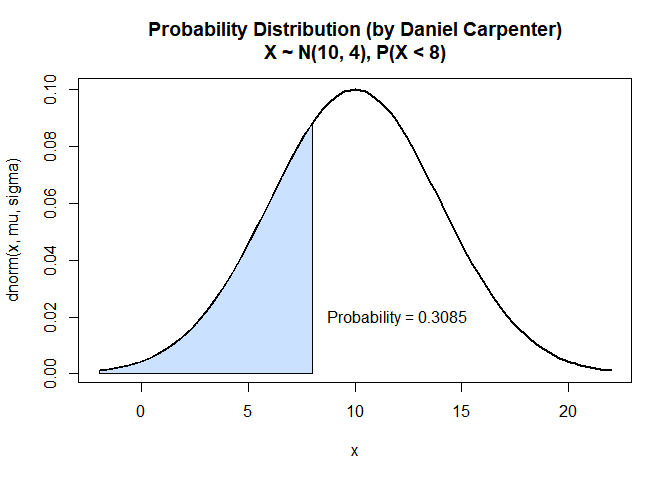
\includegraphics{lab3_files/figure-latex/2a-1.pdf}

\hypertarget{b.-find-ux1d443ux1d44b-11-1}{%
\subsection{\texorpdfstring{\texttt{b.} Find 𝑃(𝑋 ≥
11)}{b. Find 𝑃(𝑋 ≥ 11)}}\label{b.-find-ux1d443ux1d44b-11-1}}

\begin{Shaded}
\begin{Highlighting}[]
\FunctionTok{Myfunction}\NormalTok{(mu, sigma, }\AttributeTok{lowerBound =} \DecValTok{11}\NormalTok{)}
\end{Highlighting}
\end{Shaded}

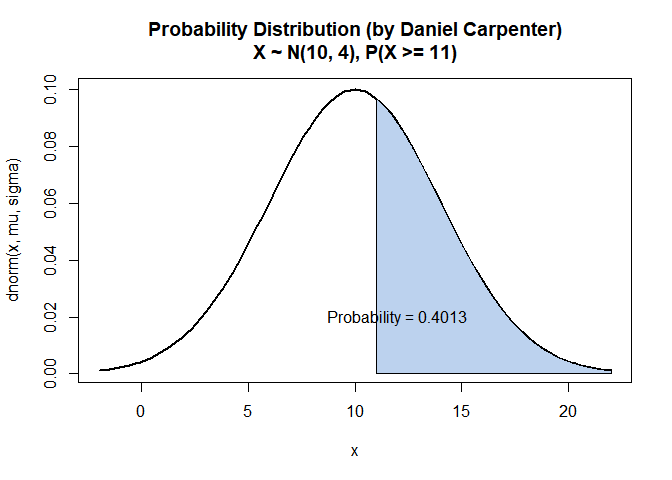
\includegraphics{lab3_files/figure-latex/2b-1.pdf}

\hypertarget{c.-find-ux1d4438-ux1d44b-14-1}{%
\subsection{\texorpdfstring{\texttt{c.} Find 𝑃(8 ≤ 𝑋 \textless{}
14)}{c. Find 𝑃(8 ≤ 𝑋 \textless{} 14)}}\label{c.-find-ux1d4438-ux1d44b-14-1}}

\begin{Shaded}
\begin{Highlighting}[]
\FunctionTok{Myfunction}\NormalTok{(mu, sigma, }\AttributeTok{lowerBound =} \DecValTok{8}\NormalTok{, }\AttributeTok{upperBound =} \DecValTok{14}\NormalTok{)}
\end{Highlighting}
\end{Shaded}

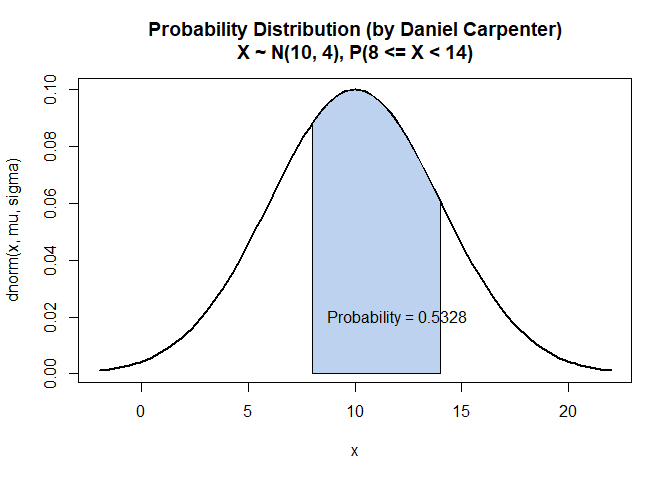
\includegraphics{lab3_files/figure-latex/2c-1.pdf}

\hypertarget{d.-find-ux1d443ux1d44b-10-1}{%
\subsection{\texorpdfstring{\texttt{d.} Find 𝑃(𝑋 \textgreater{}
10)}{d. Find 𝑃(𝑋 \textgreater{} 10)}}\label{d.-find-ux1d443ux1d44b-10-1}}

\begin{Shaded}
\begin{Highlighting}[]
\FunctionTok{Myfunction}\NormalTok{(mu, sigma, }\AttributeTok{lowerBound =} \DecValTok{10}\NormalTok{)}
\end{Highlighting}
\end{Shaded}

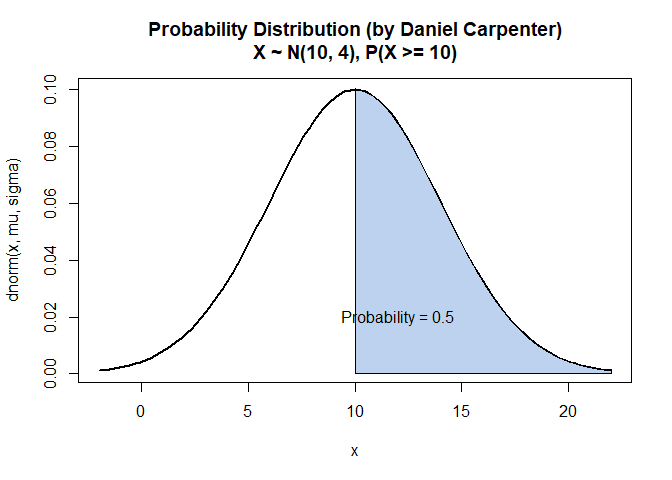
\includegraphics{lab3_files/figure-latex/2d-1.pdf}

\begin{center}\rule{0.5\linewidth}{0.5pt}\end{center}

\hypertarget{task-5-create-and-demonstrate-function-mynormplot}{%
\section{\texorpdfstring{Task \texttt{5}: Create and Demonstrate
Function
\texttt{mynormplot()}}{Task 5: Create and Demonstrate Function mynormplot()}}\label{task-5-create-and-demonstrate-function-mynormplot}}

\hypertarget{a-f-create-mynormplot-function}{%
\subsection{\texorpdfstring{\texttt{a-f} Create \texttt{mynormplot()}
Function}{a-f Create mynormplot() Function}}\label{a-f-create-mynormplot-function}}

\begin{Shaded}
\begin{Highlighting}[]
\CommentTok{\# Get function from above since it is dynamic and can handle the below calculations}
\NormalTok{mynormplot }\OtherTok{\textless{}{-}}\NormalTok{ Myfunction}
\end{Highlighting}
\end{Shaded}

\hypertarget{g.-calculate-ux1d4437-ux1d44b-10-where-ux1d44b-ux1d44185-with-mynormplot-function}{%
\subsection{\texorpdfstring{\texttt{g.} Calculate 𝑃(7 ≤ 𝑋 ≤ 10), where 𝑋
∼ 𝑁(8,5) with \texttt{mynormplot()}
Function}{g. Calculate 𝑃(7 ≤ 𝑋 ≤ 10), where 𝑋 ∼ 𝑁(8,5) with mynormplot() Function}}\label{g.-calculate-ux1d4437-ux1d44b-10-where-ux1d44b-ux1d44185-with-mynormplot-function}}

\begin{Shaded}
\begin{Highlighting}[]
\FunctionTok{mynormplot}\NormalTok{(}
  
  \CommentTok{\# Stats for Normal Distribution Creation}
  \AttributeTok{mu =} \DecValTok{8}\NormalTok{, }
  \AttributeTok{sigma =} \DecValTok{5}\NormalTok{, }
  
  \CommentTok{\# Bounds for Calculating Probability}
  \AttributeTok{lowerBound =} \DecValTok{7}\NormalTok{, }
  \AttributeTok{upperBound =} \DecValTok{10}\NormalTok{, }
  
  \CommentTok{\# Round to 6 decimal places}
  \AttributeTok{roundTo =} \DecValTok{6}\NormalTok{, }
  
  \CommentTok{\# Set color of the prob. area to "Blue"}
  \AttributeTok{color =} \StringTok{"Blue"}\NormalTok{,}
  
  \CommentTok{\# Since TRUE, we will return command line output with}
  \CommentTok{\# mean of the normal, the standard deviation and the probability calculated}
  \AttributeTok{returnCMD =} \ConstantTok{TRUE}\NormalTok{) }
\end{Highlighting}
\end{Shaded}

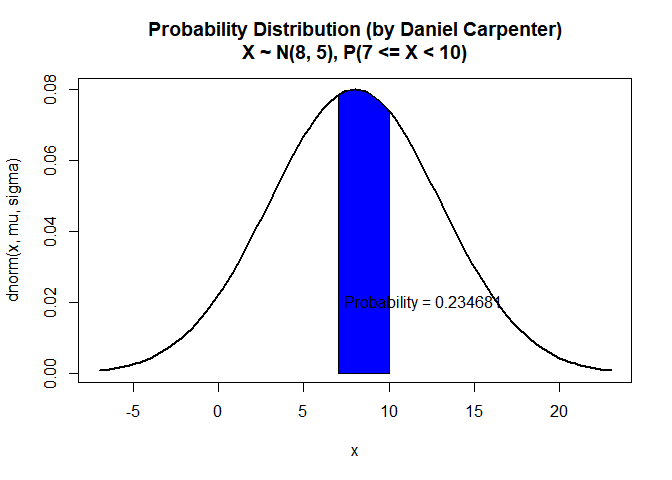
\includegraphics{lab3_files/figure-latex/5g-1.pdf}

\begin{verbatim}
## $mu
## [1] 8
## 
## $sigma
## [1] 5
## 
## $prob
## [1] 0.234681
\end{verbatim}

\begin{center}\rule{0.5\linewidth}{0.5pt}\end{center}

\hypertarget{task-6}{%
\section{\texorpdfstring{Task \texttt{6}:}{Task 6:}}\label{task-6}}

Formula for Normal Density using \(\LaTeX: \ \ X \sim N(\mu, \sigma)\)

\begin{center}\rule{0.5\linewidth}{0.5pt}\end{center}

\hypertarget{task-7}{%
\section{\texorpdfstring{Task \texttt{7}:}{Task 7:}}\label{task-7}}

\begin{Shaded}
\begin{Highlighting}[]
\ControlFlowTok{if}\NormalTok{(}\SpecialCharTok{!}\FunctionTok{require}\NormalTok{(ggplot2)) }\FunctionTok{install.packages}\NormalTok{(}\StringTok{"ggplot2"}\NormalTok{)}
\end{Highlighting}
\end{Shaded}

\begin{verbatim}
## Warning in register(): Can't find generic `scale_type` in package ggplot2 to
## register S3 method.
\end{verbatim}

\begin{Shaded}
\begin{Highlighting}[]
\FunctionTok{ggplot}\NormalTok{(}\AttributeTok{data =} \ConstantTok{NULL}\NormalTok{, }\FunctionTok{aes}\NormalTok{(}\FunctionTok{c}\NormalTok{(}\SpecialCharTok{{-}}\DecValTok{10}\NormalTok{,}\DecValTok{10}\NormalTok{))) }\SpecialCharTok{+}
  
  \CommentTok{\# LHS of the distribution (Red)}
  \FunctionTok{geom\_area}\NormalTok{(}\AttributeTok{stat =} \StringTok{"function"}\NormalTok{, }
            \AttributeTok{fun =}\NormalTok{ dnorm, }
            \AttributeTok{args =} \FunctionTok{list}\NormalTok{(}\AttributeTok{mean =} \DecValTok{0}\NormalTok{, }\AttributeTok{sd =} \DecValTok{3}\NormalTok{),}
            \AttributeTok{fill =} \StringTok{"red"}\NormalTok{, }\AttributeTok{xlim =} \FunctionTok{c}\NormalTok{(}\SpecialCharTok{{-}}\DecValTok{10}\NormalTok{, }\DecValTok{0}\NormalTok{))  }\SpecialCharTok{+} 
  
  \CommentTok{\# RHS of the distribution (Blue)}
  \FunctionTok{geom\_area}\NormalTok{(}\AttributeTok{stat =} \StringTok{"function"}\NormalTok{, }
            \AttributeTok{fun =}\NormalTok{ dnorm, }
            \AttributeTok{args =} \FunctionTok{list}\NormalTok{(}\AttributeTok{mean =} \DecValTok{0}\NormalTok{, }\AttributeTok{sd =} \DecValTok{3}\NormalTok{),}
            \AttributeTok{fill =} \StringTok{"blue"}\NormalTok{, }\AttributeTok{xlim =} \FunctionTok{c}\NormalTok{(}\DecValTok{0}\NormalTok{, }\DecValTok{10}\NormalTok{))  }\SpecialCharTok{+} 
  
  \CommentTok{\# Labels on the chart}
  \FunctionTok{labs}\NormalTok{(}\AttributeTok{title =} \StringTok{"Daniel Carpenter"}\NormalTok{,}
       \AttributeTok{subtitle =} \StringTok{"Normal Distribution with ggplot"}\NormalTok{)}
\end{Highlighting}
\end{Shaded}

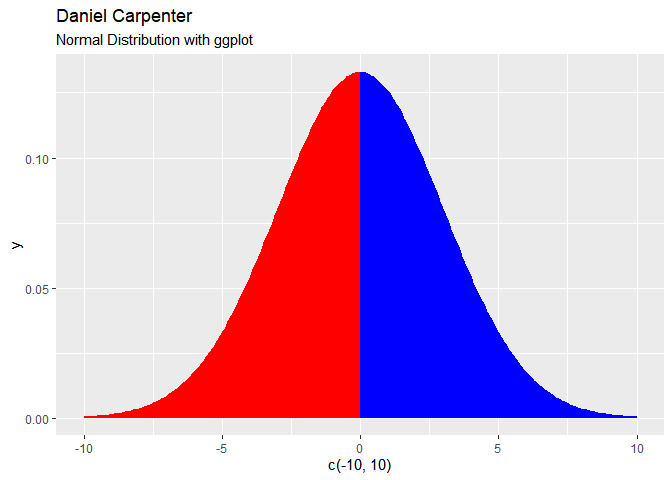
\includegraphics{lab3_files/figure-latex/ggplot-1.pdf}

\end{document}
